
\chapter{Introduction}
Droplet impact is a phenomenon which is prevalent in many industrial applications such ink-jet printing, 
spray cooling of hot surfaces. Microelectronic industries uses precision solder drop dispensing to produce
electric circuits. Aircraft and power lines encounter accumulation of ice which involves droplet impacts.
Natural phenomena such as rain effects the aeration of lakes, seas and oceans. 
Forensic science also require development of non-wettable and fully wettable surfaces. Criminalistics involves
reconstructing crimes in which it is needed to study the stain patterns of blood drops impacted on the
surface.

\begin{figure}[tbp]
 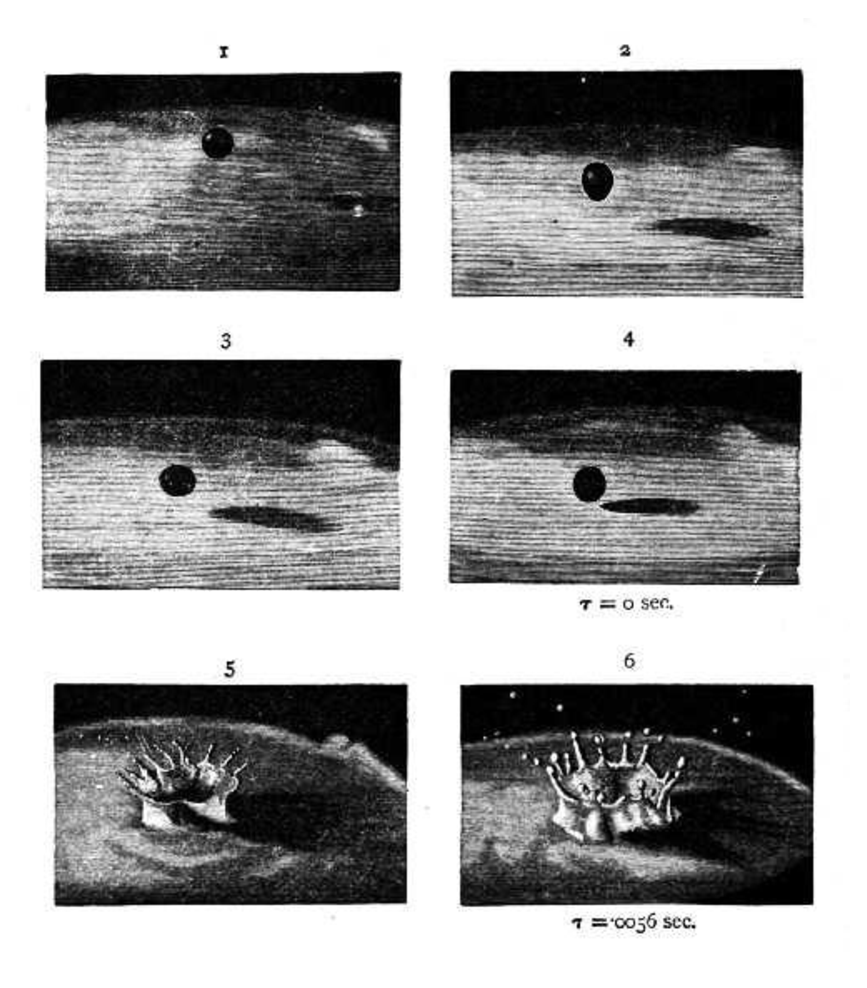
\includegraphics{worthington.eps}
 \caption[Droplet impact graphic by Worthington]{Droplet Impact from a high speed camera(Reproduced from Study of splashes by A.M Worhtington under fair usage policy)}
\end{figure}


The scientific literature on drops starts with the droplet formation which was studied by many scientists while studying the
free surface flow. The first scientific observation on drops can be found in the book by \cite{Mariotte1700} on motion of  
fluids. He observed that the water flowing through a hole of a container bottom breaks into drops. \cite{Taylor1963} solved the  axisymmetric Navier-Stokes  using
singular perturbation method for a drop/bubble in an unbounded fluid. Droplet impact was first investigated by \cite{Worthington1908} (See Fig. 1.1).
The area of droplet formation has also been researched by scientists working in the non-linear dynamics.

The dynamics of the impinging drop is complex and hence many aspects are not understood well. For example, droplets falling
on a surface can undergo many different modes of deformation. It can splash, bounce or simply deposits on a surface. \cite{Rein2002} 
explained through a cartoon, the various possibile outcomes of droplet impact. (See Fig. 1.2)

\begin{figure}[tbp]
 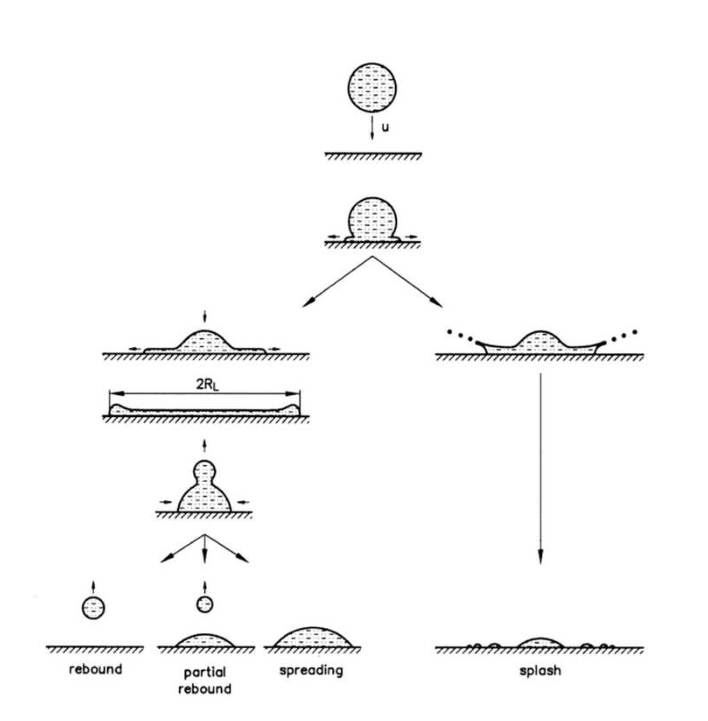
\includegraphics{rein.eps}
 \caption[Different modes of deformation of droplet impact]{Cartoon of different modes of deformation of droplet impact, reproduced from \cite{Rein2002} under fair usage policy}
\end{figure}
